\documentclass[fontset=windows]{article}
\usepackage[]{ctex}

\title{LSM Tree实验报告模板}
\author{江学强 120037910023 }
\date{4月13日 2021年}

\usepackage{natbib}
\usepackage{graphicx}
\usepackage{enumitem}
\begin{document}

\maketitle

\section{背景介绍}
这部分应该写LSM Tree这个Project的背景知识和你对这个Project的一些初步理解。 下面是教你如何在 \LaTeX 中插入一张图片。
这是一个对图片的引用, 图~\ref{fig:universe}。
\begin{figure}[h!]
\centering
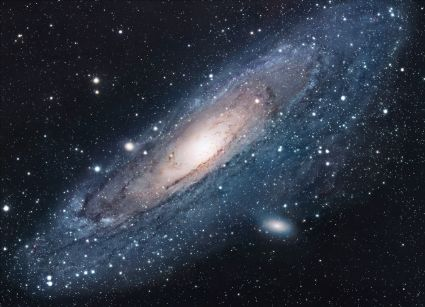
\includegraphics[scale=1.7]{universe}
\caption{The Universe}
\label{fig:universe}
\end{figure}

\section{挑战}
这部分应该叙述你在做LSM Tree Project中遇到的种种困难、挑战、bug、甚至于吐槽。


\section{测试}
此部分主要是展现你实现的项目的测试,主要分为下面几个子部分。测试部分应当是文字加上测试数据的图片展示。


\subsection{性能测试}

\subsubsection{预期结果}

在给定下面几个测试的具体数据之前,你应当首先在本节在理论上分析这些测量的结果,此步无需定量,是定性分析,
如果此处的分析与后面的具体数据测试有出入,请你给出你理解的导致这种出入的可能性。

\subsubsection{常规分析}


\begin{enumerate}
    \item 包括Get、Put、Delete操作的延迟,你需要测出不同数据大小时的操作延迟,为了测试的合理性,你应当对每个数据大小测量然后计算出平均延迟
    \item 包括Get、Put、Delete操作的吞吐,意思是指系统单位时间内能够相应的请求的次数,显然,在展示你测试的时候你需要指明Key、Value的大小(注意是数据的大小,并不是具体的值)
\end{enumerate}


\subsubsection{索引缓存与Bloom Filter的效果测试}
需要对比下面三种情况GET操作的平均时延
\begin{enumerate}
    \item 内存中没有缓存SSTable的任何信息,从磁盘中访问SSTable的索引,在找到offset之后读取数据
    \item 内存中只缓存了SSTable的索引信息,通过二分查找从SSTable的索引中找到offset,并在磁盘中读取对应的值
    \item 内存中缓存SSTable的Bloom Filter和索引,先通过Bloom Filter判断一个键值是否可能在一个SSTable中,如果存在再利用二分查找,否则直接查看下一个SSTable的索引
\end{enumerate}

\subsubsection{Compaction的影响}
不断插入数据的情况下,统计每秒钟处理的PUT请求个数(即吞吐量),并绘制其随时间变化的折线图,测试需要表现出compaction对吞吐量的影响。可以让键值对中value占用的空间大一些,从而提高compaction的频率,这样效果比较明显
\section{结论}
叙述你在做这个project过程中的收获,我们还希望能够看到你们的一些建议

\end{document}
